% А. П. Киселёв, «Элементарная геометрия», 23-е издание, 1914. Печатные с. 1–8.
\chapter*{Введение}
\addcontentsline{toc}{chapter}{Введение}

\section*{Математические предложения}
\addcontentsline{toc}{section}{Математические предложения}

% Печатная с. 1.
\kiselevparagraph{para:intro-mathematical-statements} В любой математической науке могут встретиться следующие предложения:

\textbf{Определения.} Так называют предложения, в которых разъясняется, какой смысл придают тому или другому выражению или названию. Например, в арифметике мы встречаем определения наименьшего кратного, общего наибольшего делителя и т.~п.

\textbf{Аксиомы.} Так называют истины, которые, вследствие своей очевидности, принимаются без доказательства. Таковы, например, предложения:

Если каждая из двух величин равна одной и той же третьей величине, то эти две величины равны между собой.

Если к равным величинам прибавим одну и ту же величину или вычтем из них одну и ту же величину, то равенство не нарушится.

Если к неравным величинам прибавим одну и ту же величину или вычтем из них одну и ту же величину, то направление неравенства не изменится, т.~е. большая величина останется большей.

\textbf{Теоремы.} Так называются предложения, истинность которых устанавливается только рассуждением (доказательством). Примером может служить арифметическая истина: «если сумма цифр делится на~9, то число делится на~9».

\textbf{Следствия.} Так называются предложения, которые составляют непосредственный вывод из аксиомы или теоремы. Например, из теоремы: «в пропорции произведение крайних членов равно произведению средних», выводится следствие: «крайний член пропорции равен произведению средних членов, делённому на другой крайний».

% Печатная с. 2.
\kiselevparagraph{para:intro-theorem-structure} \textbf{Состав теоремы.} В любой теореме можно выделить две части: условие и заключение. \emph{Условие} выражает то, что предполагается данным; \emph{заключение} --- то, что требуется доказать. Например, в теореме: «если сумма цифр делится на~9, то число делится на~9», условием служит первая часть теоремы: «\emph{если} сумма цифр делится на~9», а заключением --- вторая часть: «\emph{то} число делится на~9»; другими словами, нам дано, что сумма цифр некоторого числа делится на~9, а требуется доказать, что в таком случае и само число делится на~9.

Условие и заключение теоремы могут иногда состоять из нескольких отдельных условий и заключений; например, в теореме: «\emph{если число делится на~2 и на~3}, то оно разделится на~6», условие состоит из двух частей: если число делится на~2 и если число делится на~3.

Любую теорему можно сформулировать так, чтобы её условие начиналось со слова «если», а заключение --- со слова «то».

\kiselevparagraph{para:intro-converse-theorem} \textbf{Обратная теорема.} Теоремой, обратной данной теореме, называется такая, в которой условием служит заключение или часть заключения данной теоремы, а заключением --- условие или часть условия данной теоремы. Например, следующие две теоремы обратны друг другу:

\begin{center}
    \begin{tabular}{@{}p{0.44\linewidth}|p{0.44\linewidth}@{}}
        \emph{Если} сумма цифр делится на~9,\par \emph{то} число делится на~9. &
        \emph{Если} число делится на~9,\par \emph{то} сумма цифр делится на~9.
    \end{tabular}
\end{center}

Если одну из этих теорем назовём \emph{прямой}, то другую следует назвать \emph{обратной}.

В этом примере обе теоремы, и прямая и обратная, оказываются верными. Но так бывает не всегда. Например, теорема: «если каждое слагаемое делится на одно и то же число, то и сумма разделится на то же число» --- верна, но неверно обратное предложение: «если сумма делится на какое-нибудь число, то каждое слагаемое разделится на него».

\kiselevparagraph{para:intro-opposite-theorem} \textbf{Противоположная теорема.} Теоремой, противоположной данной теореме, называется такая, условие и заключение которой представляют \emph{отрицание} условия и заключения
% Печатная с. 3.
данной теоремы. Например, теореме: «если сумма цифр делится на~9, то число делится на~9» соответствует такая противоположная: «если сумма цифр \textbf{не} делится на~9, то число \textbf{не} делится на~9».

Здесь также следует заметить, что верность прямой теоремы ещё не служит признаком верности противоположной; например, противоположное предложение: «если каждое слагаемое \emph{не} делится на одно и то же число, то и сумма \emph{не} разделится на это число», --- неверно, тогда как прямое предложение верно.

\kiselevparagraph{para:intro-relations-between-theorems} \textbf{Зависимость между теоремами: прямой, обратной и противоположной.} Чтобы лучше понять эту зависимость, запишем теоремы в сокращённом виде:

\begin{enumerate}[label=\arabic*),ref=\arabic*]
    \item\label{item:direct-theorem} \emph{Прямая теорема:} если есть \(A\), то есть и \(B\).
    \item\label{item:converse-theorem} \emph{Обратная теорема:} если есть \(B\), то есть и \(A\).
    \item\label{item:opposite-direct-theorem} \emph{Противоположная прямой:} если нет \(A\), то нет и \(B\).
    \item\label{item:opposite-converse-theorem} \emph{Противоположная обратной:} если нет \(B\), то нет и \(A\).
\end{enumerate}

Легко заметить, что \hyperref[item:direct-theorem]{первое} и \hyperref[item:opposite-converse-theorem]{четвёртое} предложения \emph{следуют друг из друга}, как и \hyperref[item:converse-theorem]{второе} и \hyperref[item:opposite-direct-theorem]{третье}. Действительно, из предложения «если есть \(A\), то есть и \(B\)» непосредственно следует «если нет \(B\), то нет и \(A\)» (так как если бы \(A\) было, то, согласно \hyperref[item:direct-theorem]{первому предложению}, было бы и \(B\)). И наоборот, из предложения «если нет \(B\), то нет и \(A\)» выводим «если есть \(A\), то есть и \(B\)» (так как если бы \(B\) не было, то не было бы и \(A\)). Точно так же можно убедиться, что из \hyperref[item:converse-theorem]{второго предложения} следует \hyperref[item:opposite-direct-theorem]{третье}, и наоборот.

Поэтому, чтобы быть уверенным в верности всех четырёх теорем, достаточно доказать две из них: прямой и обратной или прямой и противоположной.

\section*{Прямая линия, плоскость. Понятие о геометрии}
\addcontentsline{toc}{section}{Прямая линия, плоскость. Понятие о геометрии}

\kiselevparagraph{para:intro-geometric-figures} \textbf{Геометрические фигуры.} Любая ограниченная часть пространства называется \emph{геометрическим телом}.

Геометрическое тело можно подразделять \emph{на части}; каждая часть геометрического тела также является геометрическим телом.

Граница геометрического тела, т.~е. то, чем оно отделяется от остального пространства, называется \emph{поверхностью}.

% Печатная с. 4.
Поверхность можно подразделять \emph{на части}; каждая часть поверхности также является поверхностью.

Граница поверхности называется \emph{линией}.

Линию можно также подразделять \emph{на части}; каждая часть линии также является линией.

Граница линии называется \emph{точкой}.

Геометрическое тело, поверхность, линия и точка не существуют по отдельности. Однако мысленно можно рассматривать поверхность независимо от геометрического тела, линию --- независимо от поверхности и точку --- независимо от линии. При этом поверхность мы должны представлять себе не имеющей толщины, линию --- не имеющей ни толщины, ни ширины, и точку --- не имеющей ни длины, ни ширины, ни толщины.

Любая линия содержит в себе бесчисленное множество точек. Принято говорить, что эти точки \emph{лежат} на линии, или что эта линия \emph{проходит} через эти точки. Их можно рассматривать как последовательные положения одной и той же точки, движущейся вдоль этой линии. Поэтому можно сказать, что \emph{линия --- след движения точки}. Если, например, мы ведём остриём карандаша по бумаге, получившийся след можно считать линией лишь приблизительно. Остриё карандаша не является геометрической точкой, поэтому след на бумаге имеет некоторую ширину (и даже толщину). Чем острее заточен карандаш, тем ближе его остриё к геометрической точке, а проведённая им линия --- к геометрической линии.

Аналогично поверхность можно рассматривать как \emph{след движения линии}, двигающейся в пространстве некоторым образом.

Совокупность каких бы то ни было точек, линий, поверхностей или тел, расположенных известным образом в пространстве, называется вообще геометрической \emph{фигурой}.

\kiselevparagraph{para:intro-geometry} \textbf{Геометрия.} Наука, рассматривающая свойства геометрических фигур, называется \emph{геометрией}, что в переводе с
% Печатная с. 5.
греческого языка означает \emph{землемерие}. Эта наука получила такое название потому, что в древности главной целью геометрии было измерение расстояний и площадей на земной поверхности.

\kiselevparagraph{para:intro-space-axiom} В начале изучения геометрии следует указать следующее общее свойство фигур:

\textbf{Аксиома пространства. Любую геометрическую фигуру можно перенести из одного места пространства в другое, не нарушая ни величины составляющих фигуру частей, ни их взаимного расположения.}

\kiselevparagraph{para:intro-straight-line} \textbf{Прямая линия.} Каждый знает, что такое \emph{прямая линия}, или просто \emph{прямая}, представление о которой нам даёт туго натянутая нить. \emph{Понятие о прямой элементарно}, т.~е. оно не может быть определено через другие, более простые понятия.

На рисунке прямую изображают в виде тонкой черты, проведённой от руки или с помощью чертёжной \emph{линейки}.

Прямая линия обладает следующими очевидными свойствами:

\textbf{Аксиомы прямой.}

\begin{enumerate}[label=\arabic*),ref=\arabic*]
    \item\label{item:line-through-two-points} \textbf{Через любые две точки пространства можно провести ровно одну прямую.}
    \item \textbf{Прямую можно продолжать без конца в обе стороны от каждой её точки.}
\end{enumerate}

Из \hyperref[item:line-through-two-points]{первой аксиомы} следует:

Если две прямые наложены одна на другую так, что две точки одной прямой совпадают с двумя точками другой прямой, то эти прямые \emph{совпадают} и во всех остальных точках (иначе через две точки можно было бы провести две различные прямые, что противоречит \hyperref[item:line-through-two-points]{первой аксиоме}).

По той же причине две прямые могут пересечься только \emph{в одной точке}.

\kiselevparagraph{para:intro-finite-and-infinite-lines} \textbf{Прямая конечная и бесконечная.} Если прямую мысленно продолжают без конца в обе стороны, её называют \emph{бесконечной} или \emph{неограниченной} прямой. Конечно, такую прямую изобразить на рисунке
% Печатная с. 6.
невозможно. Изображают только часть прямой и представляют, что она продолжается в обе стороны без конца. Прямую обычно обозначают двумя буквами, соответствующими любым двум её точкам. Так говорят «прямая \(AB\) или \(BA\)» (рис.~\ref{fig:kiselev-intro-line}).

\begin{figure}[htbp]
    \centering
    \captionsetup{name=Рис.,labelsep=period}
    \begin{minipage}[t]{0.46\linewidth}
        \centering
        \captionsetup{type=figure}
        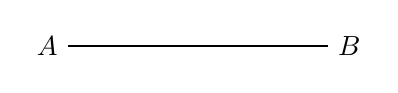
\begin{tikzpicture}
    \draw[thick] (0,0) node[left] {\(A\)} -- (3.3,0) node[right] {\(B\)};
\end{tikzpicture}

        \caption{Прямая \(AB\) или \(BA\)}
        \label{fig:kiselev-intro-line}
    \end{minipage}\hfill
    \begin{minipage}[t]{0.46\linewidth}
        \centering
        \captionsetup{type=figure}
        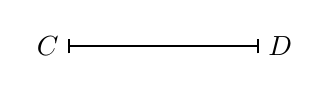
\begin{tikzpicture}
    \draw[thick] (0,0) node[left] {\(C\)} -- (2.4,0) node[right] {\(D\)};
    \draw[thick] (0,-0.09) -- (0,0.09) (2.4,-0.09) -- (2.4,0.09);
\end{tikzpicture}

        \caption{Отрезок \(CD\)}
        \label{fig:kiselev-intro-segment}
    \end{minipage}
\end{figure}

Часть прямой, ограниченная с обеих сторон, называется \emph{отрезком} прямой или \emph{конечной} прямой; такой отрезок обозначают двумя буквами у его концов (отрезок \(CD\), рис.~\ref{fig:kiselev-intro-segment}). Отрезок прямой, соединяющий две точки, называется иногда \emph{расстоянием} между ними.

Иногда рассматривают прямую, ограниченную только с одной стороны, например, в точке \(A\) (рис.~\ref{fig:kiselev-intro-ray}). О такой прямой говорят, что она \emph{исходит} из точки \(A\); её называют \emph{полупрямой} (или \emph{лучом}).

\begin{figure}[htbp]
    \centering
    \captionsetup{name=Рис.,labelsep=period}
    \begin{tikzpicture}
    \draw[thick] (0,0) node[left] {\(A\)} -- (4.2,0);
    \draw[thick] (0,-0.09) -- (0,0.09);
    \draw[thick,densely dashed] (4.2,0) -- (6,0);
\end{tikzpicture}

    \caption{Полупрямая (или луч)}
    \label{fig:kiselev-intro-ray}
\end{figure}

\kiselevparagraph{para:intro-comparison-of-segments} \textbf{Равенство и неравенство конечных прямых. Два отрезка прямой считаются равными, если они могут быть наложены друг на друга так, что совмещаются.} Допустим, что мы накладываем отрезок \(AB\) на отрезок \(CD\) (рис.~\ref{fig:kiselev-intro-sum}) так, чтобы точка \(A\) совпала с точкой \(C\), а отрезок \(AB\) был направлен от \(C\) к \(D\); если при этом концы \(B\) и \(D\) совпадут, то отрезки \(AB\) и \(CD\) считаются равными; в противном случае отрезки будут неравны, причём меньшим считается тот, который составляет часть другого.

Чтобы отложить на прямой отрезок, равный данному, пользуются \emph{циркулем} --- прибором, знакомым учащимся по опыту.

\kiselevparagraph{para:intro-sum-of-segments} \textbf{Сумма конечных прямых. Суммой нескольких данных отрезков прямой называется отрезок прямой, составленный из частей, равных соответственно данным отрезкам.} Допустим, нужно найти сумму трёх отрезков: \(AB\), \(CD\) и \(EF\) (рис.~\ref{fig:kiselev-intro-sum}). Для
% Печатная с. 7.
этого на какой-нибудь прямой берём произвольную точку \(M\) и откладываем от неё часть \(MN\), равную \(AB\); затем от точки \(N\) в том же направлении откладываем часть \(NP\), равную \(CD\), и часть \(PQ\), равную \(EF\). Отрезок \(MQ\) будет суммой данных отрезков \(AB\), \(CD\) и \(EF\), которые по отношению к этой сумме называются слагаемыми. Подобным образом можно получить сумму какого угодно числа отрезков.

\begin{figure}[htbp]
    \centering
    \captionsetup{name=Рис.,labelsep=period}
    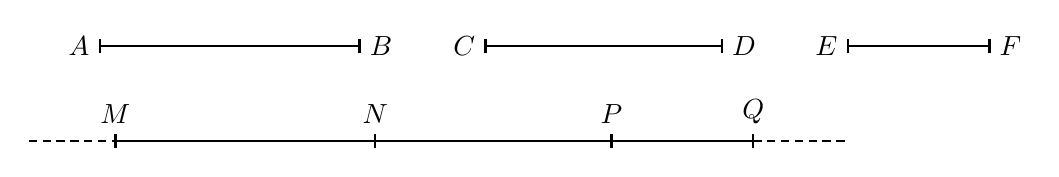
\begin{tikzpicture}
    \foreach \leftlabel/\rightlabel/\first/\last in {A/B/0/3.3,C/D/4.9/7.9,E/F/9.5/11.3} {
        \draw[thick] (\first,1.2) node[left] {\(\leftlabel\)}
            -- (\last,1.2) node[right] {\(\rightlabel\)};
        \draw[thick] (\first,1.11) -- (\first,1.29) (\last,1.11) -- (\last,1.29);
    }
    \draw[thick] (0.2,0) -- (8.3,0);
    \draw[thick,densely dashed] (-0.9,0) -- (0.2,0) (8.3,0) -- (9.5,0);
    \foreach \position/\point in {0.2/M,3.5/N,6.5/P,8.3/Q} {
        \draw[thick] (\position,-0.09) -- (\position,0.09) node[above] {\(\point\)};
    }
\end{tikzpicture}

    \caption{Сумма конечных прямых}
    \label{fig:kiselev-intro-sum}
\end{figure}

Сумма отрезков прямой обладает теми же свойствами, что и любая сумма. Она не зависит от порядка слагаемых (\emph{переместительное свойство}) и не изменяется, если некоторые слагаемые заменить их суммой (\emph{сочетательное свойство}). Например, легко убедиться (рис.~\ref{fig:kiselev-intro-sum}), что
\[
    \begin{gathered}
        AB+CD+EF=CD+EF+AB=EF+AB+CD=\dots \\
        \text{и}\quad AB+CD+EF=AB+(CD+EF).
    \end{gathered}
\]

Из понятия о сумме выводятся понятия о разности, произведении и частном отрезков. Так, \emph{разность} отрезков \(AB\) и \(CD\) (если \(AB>CD\)) --- это отрезок, который в сумме с \(CD\) даёт \(AB\); \emph{произведение} отрезка \(AB\) на число~3 равно сумме трёх отрезков, из которых каждый равен \(AB\), \emph{частное} при делении отрезка \(AB\) на число~3 равно третьей части \(AB\) и т.~п.

Мы считаем очевидным, что любой отрезок прямой можно разделить (хотя бы только мысленно) на~2, на~3, на~4 и т.~д. равные части.

\kiselevparagraph{para:intro-plane} \textbf{Плоскость. Плоскостью называется поверхность, обладающая тем свойством, что прямая, проходящая через любые две точки этой поверхности, целиком лежит на этой поверхности.} Допустим, мы хотим проверить, является ли поверхность стола плоскостью. Для этого берём хорошо выверенную линейку и прикладываем её краем в различных направлениях к поверхности стола так, чтобы какие-нибудь
% Печатная с. 8.
две точки линейки лежали на этой поверхности. Если при этом окажется, что, в каком бы направлении мы ни приложили линейку, все остальные её точки будут лежать на поверхности стола, то эта поверхность является плоскостью.

Существование плоскости в пространстве принимается за аксиому.

Укажем следующее свойство плоскости, которое мы примем здесь без доказательства:

\textbf{Любую часть плоскости можно наложить всеми её точками на другое место этой или другой плоскости, причём накладываемую часть можно предварительно перевернуть на другую сторону.}

\kiselevparagraph{para:intro-branches-of-geometry} \textbf{Разделение геометрии.} Геометрия делится на две части: \emph{планиметрия} и \emph{стереометрия}. Первая рассматривает свойства фигур, все части которых лежат в одной плоскости. Вторая рассматривает свойства фигур, не все части которых лежат в одной плоскости.
